\chapter{Business model by Unified Modeling Language}
\section{General Usecase Diagram}
\begin{figure}[H] % [h] giúp đặt ảnh tại vị trí bạn viết code
    \centering % Căn lề giữa cho ảnh
    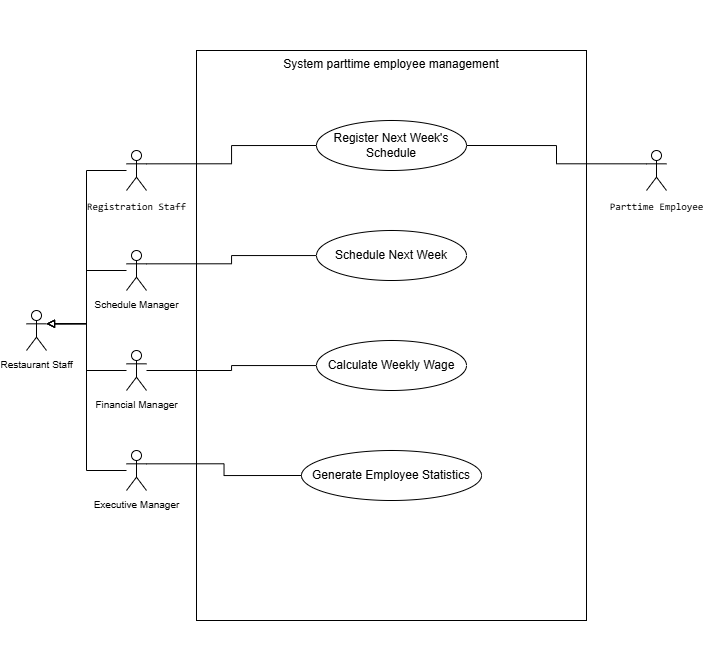
\includegraphics[width=0.8\textwidth]{assets/diagrams/general-usecase.png}
    \caption{
Usecase General Diagram for the Parttime Management System}
    % \label{fig:anh_vi_du} 
\end{figure}
\section{Usecase General Diagram for the Parttime Management System}

\begin{itemize}
    \item This use case enables the Registration Staff to Register Next Week's Schedule upon the request of the Parttime Employee.
    \item This use case enables the Schedule Manager to Schedule Next Week.
    \item This use case enables the Financial Manager to Calculate Weekly Wage.
    \item This use case enables the Executive Manager to Generate Employee Statistics.
\end{itemize}

\section{Detail Usecase Diagram}

\subsection{Detail Usecase Diagram}
\begin{figure}[H]
    \centering
    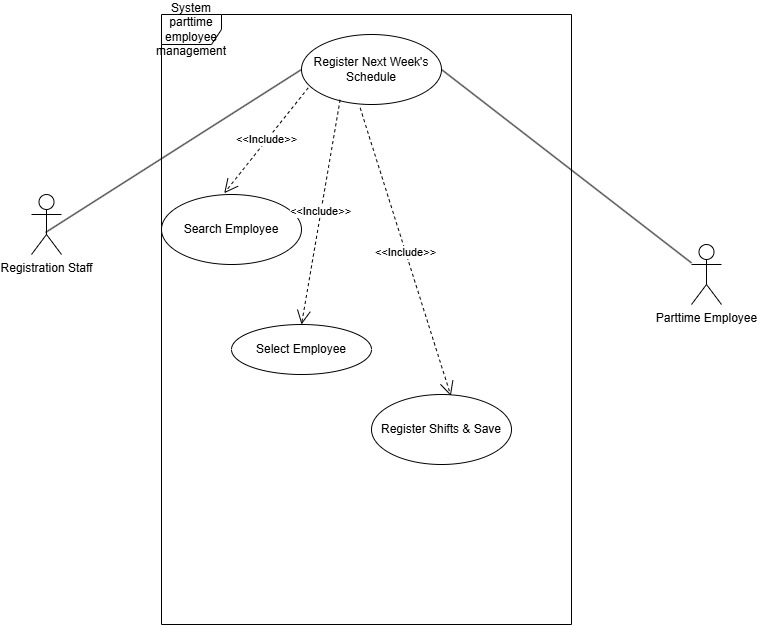
\includegraphics[width=0.8\textwidth]{assets/diagrams/Detail Use Case.jpg}
    \caption{Detail Usecase Diagram for the Parttime Management System}
    % \label{fig:detail_usecase}
\end{figure}

\subsection{Use Case Description}

\begin{itemize}
    \item This use case allows the Registration Staff to register the next week's working schedule on the system under the influence/request of the Parttime Employee.

    \item This use case allows the Registration Staff to search for employee information on the system under the request of the Parttime Employee.

    \item This use case allows the Registration Staff to select exactly one employee from the search result list.

    \item This use case allows the Registration Staff to select working shifts and save the next week's schedule registration information for the selected employee.
\end{itemize}

\section{Scenario}

\renewcommand{\arraystretch}{1.5}
\begin{longtable}{|p{3cm}|p{13cm}|}
\hline
\textbf{Scenario} & Register for Next Week (Register next week's working shifts) \\
\hline
\textbf{Actor} & Registration Staff, Parttime Employee \\
\hline
\textbf{Pre-condition} &
\begin{itemize}
    \item Registration Staff has a valid staff account in the system.
    \item The current time is before the next week's schedule is finalized (before the registration deadline).
    \item The current Minimum Shift Threshold = 3 shifts/week.
\end{itemize} \\
\hline
\textbf{Post-condition} & The next week's shift registration of the employee is successfully saved into the database. \\
\hline

% === Main Events: Part 1 (Steps 1-10 with search result table) ===
\textbf{Main Events} &
\begin{enumerate}
    \item Staff A opens the system login interface.
    \item Staff A enters username and password and clicks the ``Login'' button.
    \item The system checks the login information.
    \item The login is successful, and the system displays the staff home page.
    \item Staff A selects the function to register working shifts for next week on the system upon the request of Parttime Employee B directly at the restaurant.
    \item The system displays the Employee Search Interface, which includes a text field with the placeholder ``Enter employee name...'' and a ``Search'' button.
    \item Staff A asks Parttime Employee B for their full name to search on the system.
    \item Parttime Employee B provides the name: ``B''.
    \item Staff A enters the keyword ``B'' into the search field and clicks the ``Search'' button.
    \item The system queries the database, finds all employees whose names contain the keyword ``B'', and displays the Employee Search Result List on the interface as the following table:

    \begin{tabular}{|c|c|c|c|}
    \hline
    \textbf{No.} & \textbf{Employee Code} & \textbf{Employee Name} & \textbf{Phone Number} \\
    \hline
    1 & B23DCCE060 & B & 0912345678 \\
    \hline
    2 & B23DCCE088 & Binh & 0987654321 \\
    \hline
    \end{tabular}
\end{enumerate} \\
\hline

% === Main Events: Part 2 (Steps 11-14 with empty registration table) ===
\textbf{Main Events (cont.)} &
\begin{enumerate}
    \setcounter{enumi}{10}
    \item Staff A informs Parttime Employee B that the system found 2 results and reads the list for confirmation.
    \item Parttime Employee B confirms that row number 1 - ``B'' - is correct.
    \item Staff A clicks on row number 1 ``B'' in the list.
    \item The system displays the Register Shift Interface, which includes: the selected employee's information and the next week's registration table (7 rows $\times$ 2 checkbox columns).

    \begin{tabular}{|c|c|c|c|c|}
    \hline
    \textbf{No.} & \textbf{Day} & \textbf{Date} & \textbf{Shift 1} & \textbf{Shift 2} \\
    \hline
    1 & Monday & 24/03/2026 & & \\
    \hline
    2 & Tuesday & 25/03/2026 & & \\
    \hline
    3 & Wednesday & 26/03/2026 & & \\
    \hline
    4 & Thursday & 27/03/2026 & & \\
    \hline
    5 & Friday & 28/03/2026 & & \\
    \hline
    6 & Saturday & 29/03/2026 & & \\
    \hline
    7 & Sunday & 30/03/2026 & & \\
    \hline
    \end{tabular}
\end{enumerate} \\
\hline

% === Main Events: Part 3 (Steps 15-17 with filled registration table) ===
\textbf{Main Events (cont.)} &
\begin{enumerate}
    \setcounter{enumi}{14}
    \item Staff A asks Parttime Employee B which shifts they want to register for next week.
    \item Parttime Employee B replies that they want to register: Shift 1 on Monday, Shift 2 on Wednesday, Shift 1 on Friday, and Shift 2 on Saturday (a total of 4 shifts).
    \item Staff A checks the corresponding checkboxes and clicks the ``Save'' button. The table becomes:

    \begin{tabular}{|c|c|c|c|c|}
    \hline
    \textbf{No.} & \textbf{Day} & \textbf{Date} & \textbf{Shift 1} & \textbf{Shift 2} \\
    \hline
    1 & Monday & 24/03/2026 & x & \\
    \hline
    2 & Tuesday & 25/03/2026 & & \\
    \hline
    3 & Wednesday & 26/03/2026 & & x \\
    \hline
    4 & Thursday & 27/03/2026 & & \\
    \hline
    5 & Friday & 28/03/2026 & x & \\
    \hline
    6 & Saturday & 29/03/2026 & & x \\
    \hline
    7 & Sunday & 30/03/2026 & & \\
    \hline
    \end{tabular}
\end{enumerate} \\
\hline

% === Main Events: Part 4 (Steps 18-20) ===
\textbf{Main Events (cont.)} &
\begin{enumerate}
    \setcounter{enumi}{17}
    \item The system performs validation: counts the total number of checked checkboxes = 4 shifts. Compares with Minimum Shift Threshold = 3 shifts. Result: 4 $\geq$ 3 $\rightarrow$ Valid.
    \item The system saves the next week's shift registration information of Employee B into the database and displays the notification: ``Registration successfully saved!''.
    \item Staff A informs Parttime Employee B that the next week's shift registration has been completed successfully.
\end{enumerate} \\
\hline

% === Exception 4a ===
\textbf{Exception} &
\textbf{Exception 4a: Login information is incorrect}
\begin{enumerate}
    \item[4.1.] Instead of displaying the home page, the system displays the warning: ``Invalid username or password.''
    \item[4.2.] Staff A re-enters username and password and clicks the ``Login'' button again.
    \item[4.3.] The system checks the login information again. If the information is valid, the system displays the staff home page similar to step 4 of the main scenario.
\end{enumerate} \\
\hline

% === Exception 9a ===
\textbf{Exception (cont.)} &
\textbf{Exception 9a: Search field is empty}
\begin{enumerate}
    \item[9.1.] The system displays a warning on the interface: ``Please enter the search keyword.''
    \item[9.2.] Staff A asks Parttime Employee B to provide the name again.
    \item[9.3.] Parttime Employee B provides the name again: ``B''.
    \item[9.4.] Staff A enters ``B'' into the search field and clicks the ``Search'' button.
    \item[9.5.] The result appears similar to step 10 of the main scenario.
\end{enumerate} \\
\hline

% === Exception 9b ===
\textbf{Exception (cont.)} &
\textbf{Exception 9b: Search field is empty, employee refuses to provide again}
\begin{enumerate}
    \item[9.1.] The system displays a warning: ``Please enter the search keyword.''
    \item[9.2.] Staff A asks Parttime Employee B to provide the name again.
    \item[9.3.] Parttime Employee B refuses to provide information.
    \item[9.4.] Staff A closes the registration interface. The system returns to the home page. $\rightarrow$ End.
\end{enumerate} \\
\hline

% === Exception 10a ===
\textbf{Exception (cont.)} &
\textbf{Exception 10a: No employee found, employee provides again}
\begin{enumerate}
    \item[10.1.] The system displays the message: ``No employee found.''
    \item[10.2.] Staff A informs Parttime Employee B that no employee was found, and asks if they want to try again.
    \item[10.3.] Parttime Employee B provides a different name.
    \item[10.4.] Staff A enters ``B'' into the search field and clicks the ``Search'' button.
    \item[10.5.] The result with employees appears similar to step 10 of the main scenario.
\end{enumerate} \\
\hline

% === Exception 10b ===
\textbf{Exception (cont.)} &
\textbf{Exception 10b: No employee found, employee refuses to provide again}
\begin{enumerate}
    \item[10.1.] The system displays the message: ``No employee found.''
    \item[10.2.] Staff A informs Parttime Employee B that no employee was found, and asks if they want to try again.
    \item[10.3.] Parttime Employee B does not want to try again.
    \item[10.4.] Staff A closes the registration interface. The system returns to the home page. $\rightarrow$ End.
\end{enumerate} \\
\hline

% === Exception 13 ===
\textbf{Exception (cont.)} &
\textbf{Exception 13: Target employee not found in the result list}
\begin{enumerate}
    \item[13.1.] Staff A reads the result list to Parttime Employee B but cannot find the correct person.
    \item[13.2.] Staff A asks Parttime Employee B to confirm the name again or provide a more accurate name.
    \item[13.3.] Parttime Employee B provides a more accurate name: ``B''.
    \item[13.4.] Staff A clears the search field, re-enters ``B'', and clicks the ``Search'' button.
    \item[13.5.] The result with employees appears similar to step 10 of the main scenario.
\end{enumerate} \\
\hline

% === Exception 18a ===
\textbf{Exception (cont.)} &
\textbf{Exception 18a: Insufficient minimum shifts, employee supplements}
\begin{enumerate}
    \item[18.1.] The system displays a warning: ``The number of registered shifts (2) is below the minimum threshold (3). Please register at least 1 more shift.''
    \item[18.2.] Staff A informs Parttime Employee B that they need to register at least 1 more shift.
    \item[18.3.] Parttime Employee B agrees and chooses to add Shift 2 on Thursday.
    \item[18.4.] Staff A checks the additional checkbox for Shift 2 on Thursday. The table is updated, total = 3 shifts.
    \item[18.5.] Staff A clicks the ``Save'' button.
    \item[18.6.] The system validates: 3 $\geq$ 3 $\rightarrow$ Valid. Registration saved successfully, similar to step 19 of the main scenario.
\end{enumerate} \\
\hline

% === Exception 18b ===
\textbf{Exception (cont.)} &
\textbf{Exception 18b: Insufficient minimum shifts, employee refuses to supplement}
\begin{enumerate}
    \item[18.1.] The system displays a warning: ``The number of registered shifts (2) is below the minimum threshold (3). Please register at least 1 more shift.''
    \item[18.2.] Staff A informs Parttime Employee B that additional shifts are needed.
    \item[18.3.] Parttime Employee B refuses to register more shifts.
    \item[18.4.] Staff A closes the registration interface. The system does not save the data and returns to the home page. $\rightarrow$ End.
\end{enumerate} \\
\hline
\end{longtable}
\renewcommand{\arraystretch}{1}

\section{Extracting and Building the Entity Class Diagram for Module}


\subsection{System Description}

This module supports the management of part-time employee shift registration within a restaurant chain. The restaurant chain consists of multiple restaurants, and each restaurant employs many hourly employees. Each working day is divided into two fixed shifts: Shift 1 from 8:00 AM to 4:00 PM and Shift 2 from 4:00 PM to 12:00 AM. The hourly rate is applied uniformly to all employees.

After signing a valid employment contract, an employee is allowed to register his or her available working time for the following week. The number of shifts registered in each week must satisfy the prescribed Minimum Shift Threshold. The system enables a Registration Staff member to log in with a username and password, search for an employee by name, select the correct employee from the matched results, and register the employee's available shifts through a 7-day $\times$ 2-shift registration table. Before saving the registration, the system validates whether the total number of selected shifts satisfies the minimum threshold. If the validation is successful, the system records the registration data for later scheduling activities.

\subsection{Noun Extraction and Evaluation}


\renewcommand{\arraystretch}{1.35}
\begin{longtable}{|>{\centering\arraybackslash}p{0.8cm}|p{3.1cm}|p{3.2cm}|p{8.0cm}|}
\hline
\textbf{No.} & \textbf{Noun} & \textbf{Classification} & \textbf{Reasoning} \\
\hline
\endfirsthead

\hline
\textbf{No.} & \textbf{Noun} & \textbf{Classification} & \textbf{Reasoning} \\
\hline
\endhead

\hline
\endfoot

\hline
\endlastfoot

1 & System & Rejected & An abstract and general term; it does not represent a concrete business object. \\
\hline
2 & Restaurant chain & Rejected & Too broad for Module 1; the module manages employees and registrations at the restaurant level rather than modeling the whole chain as a separate entity. \\
\hline
3 & Restaurant & Entity class & Employees belong to a restaurant, so restaurant information must be represented. $\rightarrow$ Restaurant. \\
\hline
4 & Employee & Entity class & The core object of the module; employees are searched, selected, and registered for shifts. $\rightarrow$ Employee. \\
\hline
5 & Working day & Rejected & A common time concept; it is represented through the date attribute of the Shift class. \\
\hline
6 & Shift & Entity class & A specific working time slot that employees register for; it has its own date, shift number, start time, and end time. $\rightarrow$ Shift. \\
\hline
7 & Shift 1 / Shift 2 & Attribute value & These are values of the shiftNumber attribute in the Shift class, not independent entity classes. \\
\hline
8 & Hourly rate & Rejected  & A system-wide configuration value that is the same for all employees; it is not an entity class in this module. \\
\hline
9 & Contract & Attribute & In Module 1, the contract is represented by the contractDate attribute of the Employee class rather than a separate class. \\
\hline
10 & Registration & Entity class & A registration record links an employee to a shift and stores registration-specific information such as time and status. $\rightarrow$ RegistrationShift. \\
\hline
11 & Available working time & Rejected & An abstract concept represented by selected checkboxes in the registration table and registration-related attributes. \\
\hline
12 & Session & Rejected & A synonym of Shift in this context; it is already represented by the Shift class. \\
\hline
13 & Week & Rejected & A common time period; the next week can be derived from the current date and does not need to be stored as an entity class for this module. \\
\hline
14 & Minimum threshold & Rejected  & A system configuration parameter defining the minimum number of shifts per week; it is not an entity class. \\
\hline
15 & Registration staff & Entity class via User & A staff member who operates the system; represented by the User class with a role attribute. \\
\hline
16 & Name & Attribute & Represented as fullName in Employee and name in User. \\
\hline
17 & Registration table & Rejected & A user-interface element used to display and select shifts; it belongs to the View layer, not the entity layer. \\
\hline
18 & User & Entity class & A person who logs in and performs system functions. $\rightarrow$ User. \\
\hline
19 & Login & Rejected & An action performed by a user, not a data entity. \\
\hline
20 & Username & Attribute & An authentication attribute of the User class. \\
\hline
21 & Password & Attribute & An authentication attribute of the User class. \\
\hline
22 & Employee code & Attribute & A unique identifier attribute of the Employee class. \\
\hline
23 & Phone number & Attribute & A contact information attribute of the Employee class. \\
\hline
\end{longtable}
\renewcommand{\arraystretch}{1}

From the noun extraction and classification process, the initial entity classes identified for the Register Next Week module are Restaurant, Employee, Shift, RegistrationShift, and User.

\subsection{Proposed Entity Classes Summary}

The final entity classes are selected based on whether each class represents a persistent business object, participates in a meaningful relationship with other classes, and stores data required by the Register Next Week module. The class RegistrationShift is introduced as an intermediary entity because an employee can register for many shifts and a shift can be registered by many employees. Therefore, the many-to-many relationship between Employee and Shift is resolved into two one-to-many relationships through RegistrationShift. This class also records the staff member who created the registration, the registration time, and the registration status.

\renewcommand{\arraystretch}{1.35}
\begin{longtable}{|p{3.0cm}|p{3.4cm}|p{5.2cm}|p{4.2cm}|}
\hline
\textbf{Entity Class} & \textbf{Class Name} & \textbf{Key Attributes} & \textbf{Purpose} \\
\hline
\endfirsthead

\hline
\textbf{Entity Class} & \textbf{Class Name} & \textbf{Key Attributes} & \textbf{Purpose} \\
\hline
\endhead

\hline
\endfoot

\hline
\endlastfoot

Restaurant & Restaurant & restaurantName, address, description & Represents the restaurant to which employees belong. \\
\hline
Employee & Employee & code, fullName, phoneNumber, email, dob, description, contractDate & Represents the part-time employee who can be searched and registered for shifts. \\
\hline
Shift & Shift & date, shiftNumber, startDate, endDate, description & Represents a specific working shift in the next week. \\
\hline
Registration Shift & RegistrationShift & registeredTime, status, description & Represents the registration record linking an employee to a selected shift. \\
\hline
User & User & username, password, role, description & Represents the staff account that logs in and performs the registration operation. \\
\hline
\end{longtable}
\renewcommand{\arraystretch}{1}

The entity relationships are summarized as follows: one Restaurant has many Employees; one Employee may have many RegistrationShift records; one Shift may have many RegistrationShift records; and one User may create many RegistrationShift records. These relationships provide the structural basis for the Entity Class Diagram of the module.

\subsection{Entity Class Diagram}
\begin{figure}[H]
    \centering
    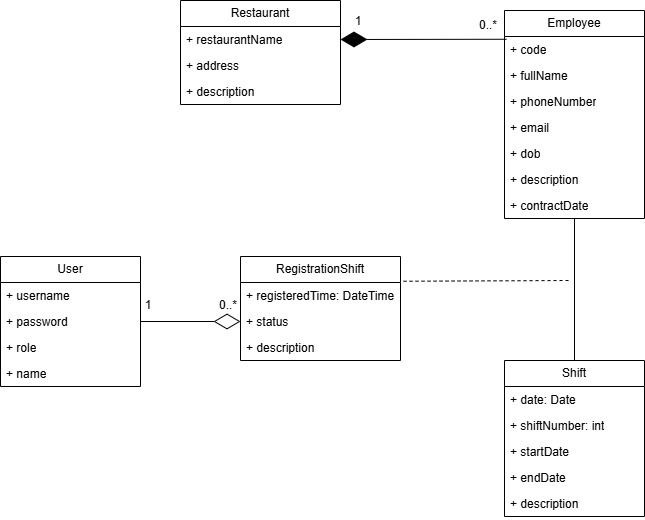
\includegraphics[width=0.9\textwidth]{assets/diagrams/Entity Classes.jpg}
    \caption{Entity Class Diagram for the Register Next Week Module}
    % \label{fig:entity_class_diagram}
\end{figure}


\section{Full Explanation and Method Identification}


\textbf{Analysis of this module:}

Enter the system $\rightarrow$ the login interface appears $\rightarrow$ need a class: LoginView.

\begin{itemize}
    \item Input for username $\rightarrow$ inUsername.
    \item Input for password $\rightarrow$ inPassword.
    \item A submit button to login $\rightarrow$ subLogin.
\end{itemize}

Enter the username/password $\rightarrow$ the system must check if the login information is correct $\rightarrow$ need a method:

\begin{itemize}
    \item Name: checkLogin().
    \item Input: username and password of the class User. In the class diagram, these data are represented by a User object.
    \item Output: boolean.
    \item Assign to the entity class: User, because the input parameters belong to the user account and this method verifies whether that account is valid.
\end{itemize}

Once login is successful $\rightarrow$ the main interface of the registration staff appears $\rightarrow$ need a class: HomepageView. This view has at least:

\begin{itemize}
    \item An option/button to choose the function Register for next week $\rightarrow$ subSearchEmployee.
\end{itemize}

Choose the option to register for next week $\rightarrow$ the search employee interface appears $\rightarrow$ need a class: SearchEmployeeView. This view is used to find the part-time employee who requests next week's shift registration.

\begin{itemize}
    \item An input text to enter the keyword for searching employee by name $\rightarrow$ inKey.
    \item A search button to execute the search $\rightarrow$ subSearch.
    \item A result table that lists matched employees and can be clicked to choose one employee $\rightarrow$ outsubListEmployee.
\end{itemize}

Enter a keyword and click Search $\rightarrow$ the system has to search all employees whose names contain the entered keyword $\rightarrow$ need a method:

\begin{itemize}
    \item Name: searchEmployee().
    \item Input: a keyword as String.
    \item Output: a list of Employee objects.
    \item Assign to the entity class: Employee, because the output of this method is a list of employees matching the search condition.
\end{itemize}

The list of matched employees will be displayed in SearchEmployeeView. The registration staff then clicks on the correct employee in the result table.

Click on an employee to register shifts $\rightarrow$ the system needs to load the shifts of the next week $\rightarrow$ need a method:

\begin{itemize}
    \item Name: getShiftNextWeek().
    \item Input: none. The method calculates the next week internally based on the current date and retrieves the corresponding shift data.
    \item Output: a list of Shift objects.
    \item Assign to the entity class: Shift, because the output of this method is the list of next-week shifts.
\end{itemize}

After the shift data is loaded $\rightarrow$ the shift registration interface appears $\rightarrow$ need a class: RegisterShiftView. This view displays the selected employee and allows the registration staff to select next week's shifts.

\begin{itemize}
    \item The selected employee's information is displayed as read-only output, including code, name, and phone number $\rightarrow$ outEmployeeInfo.
    \item A shift table with 7 rows for the next seven days and 2 columns for Shift 1 and Shift 2 is displayed. This table both shows shift information and receives checkbox input from the staff $\rightarrow$ inoutShiftTable.
    \item A save button is provided to submit the registration $\rightarrow$ subSave.
\end{itemize}

The registration staff ticks the checkboxes corresponding to the shifts that the part-time employee wants to register and clicks Save $\rightarrow$ the system has to save the registration into the database $\rightarrow$ need a method:

\begin{itemize}
    \item Name: saveRegistration().
    \item Input: an object of RegistrationShift, containing the selected employee, selected shift, user who performs the registration, registered time, and status.
    \item Output: none or boolean. In this module, boolean is used to show whether the save operation is successful.
    \item Assign to the entity class: RegistrationShift, because the input parameter is a registration object and this class represents the link between an employee and a shift.
\end{itemize}

After saving the registration successfully $\rightarrow$ the system displays a success message $\rightarrow$ the registration staff informs the part-time employee that next week's shift registration has been completed $\rightarrow$ the system returns to HomepageView.

\subsection{Identified Classes and Relationships}

From the analysis above, the View classes identified for this module are LoginView, HomepageView,\\ SearchEmployeeView, and RegisterShiftView. These classes represent the interfaces that the registration staff uses in the standard scenario.

The Entity classes involved in this module are User, Employee, Shift, RegistrationShift, and Restaurant. The class Restaurant is still included even though no method is directly assigned to it in this module, because it has a structural relationship with Employee: one restaurant has many employees.

The navigation between View classes is identified as follows. LoginView navigates to HomepageView after successful login. HomepageView navigates to SearchEmployeeView when the registration staff chooses the Register for next week function. SearchEmployeeView navigates to RegisterShiftView after the staff selects the correct employee.

The method calls between View classes and Entity classes are identified as follows. LoginView calls checkLogin() from User to verify the login information. SearchEmployeeView calls searchEmployee() from Employee to search employees by keyword. SearchEmployeeView calls getShiftNextWeek() from Shift to get the shifts for next week. RegisterShiftView calls saveRegistration() from RegistrationShift to save the selected shift registrations.

\subsection{Full Class Diagram}
\begin{figure}[H]
    \centering
    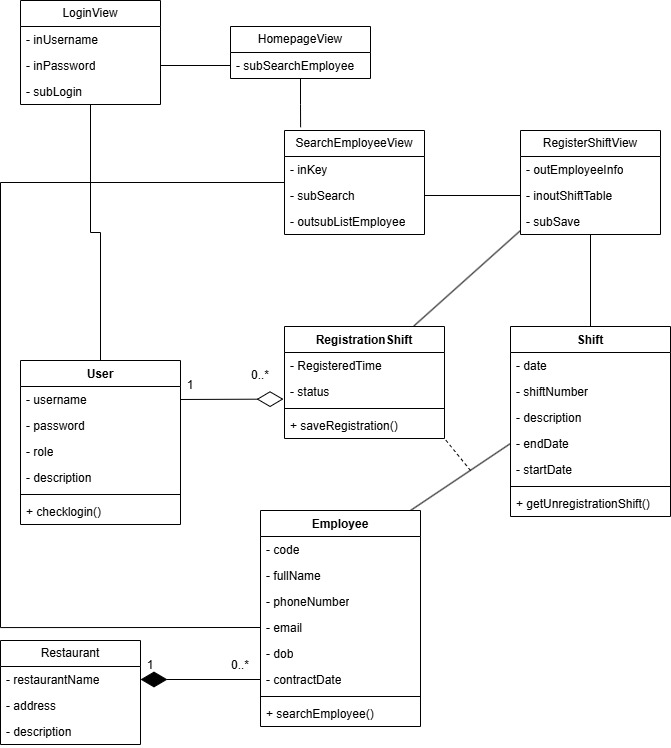
\includegraphics[width=0.9\textwidth]{assets/diagrams/Full Class Diagram.jpg}
    \caption{Full Class Diagram for the Register Next Week Module}
    % \label{fig:full_class_diagram}
\end{figure}


\section{Scenario v.2 and the Sequence Diagram for the Standard Scenario of the Module}

\subsection{Standard Scenario v.2}

\begin{enumerate}
    \item A parttime employee requests the registration staff to register next week's shifts.

    \item The registration staff enters username/password and then clicks on the Login button.

    \item The class LoginView calls the class User to process.

    \item The class User calls the method checkLogin(). The login is successful.

    \item The class User returns the results to the class LoginView.

    \item The class LoginView calls the class HomepageView.

    \item The class HomepageView displays itself to the registration staff.

    \item The registration staff chooses the option of register for next week.

    \item The class HomepageView calls the class SearchEmployeeView.

    \item The class SearchEmployeeView displays itself to the registration staff.

    \item The registration staff asks the parttime employee for his name.

    \item The parttime employee provides his name to the registration staff.

    \item The registration staff enters the employee name keyword and clicks on the search button.

    \item The class SearchEmployeeView calls the class Employee to process.

    \item The class Employee calls the method searchEmployee().

    \item The class Employee returns the results to the class SearchEmployeeView.

    \item The class SearchEmployeeView displays the list of matched employees to the registration staff.

    \item The registration staff clicks on the correct employee.

    \item The class SearchEmployeeView calls the class Shift to get the shifts of next week.

    \item The class Shift calls the method getShiftNextWeek().

    \item The class Shift returns the results to the class SearchEmployeeView.

    \item The class SearchEmployeeView calls the class RegisterShiftView with the selected employee and shift data.

    \item The class RegisterShiftView displays the employee information and the 7-day $\times$ 2-shift registration table to the registration staff.

    \item The registration staff asks the parttime employee which shifts he wants to work next week.

    \item The parttime employee provides his desired shifts to the registration staff.

    \item The registration staff ticks the checkboxes corresponding to the shifts the employee wants to register and clicks the Save button.

    \item The class RegisterShiftView calls the class RegistrationShift to process.

    \item The class RegistrationShift calls the method saveRegistration().

    \item The class RegistrationShift returns the results to the class RegisterShiftView.

    \item The class RegisterShiftView displays a successful message to the registration staff.

    \item The registration staff informs the parttime employee that the registration is successful.

    \item The registration staff clicks on the OK button of the message.

    \item The class RegisterShiftView calls the class HomepageView.

    \item The class HomepageView displays itself to the registration staff.
\end{enumerate}

\subsection{Sequence Diagram}
\begin{figure}[H]
    \centering
    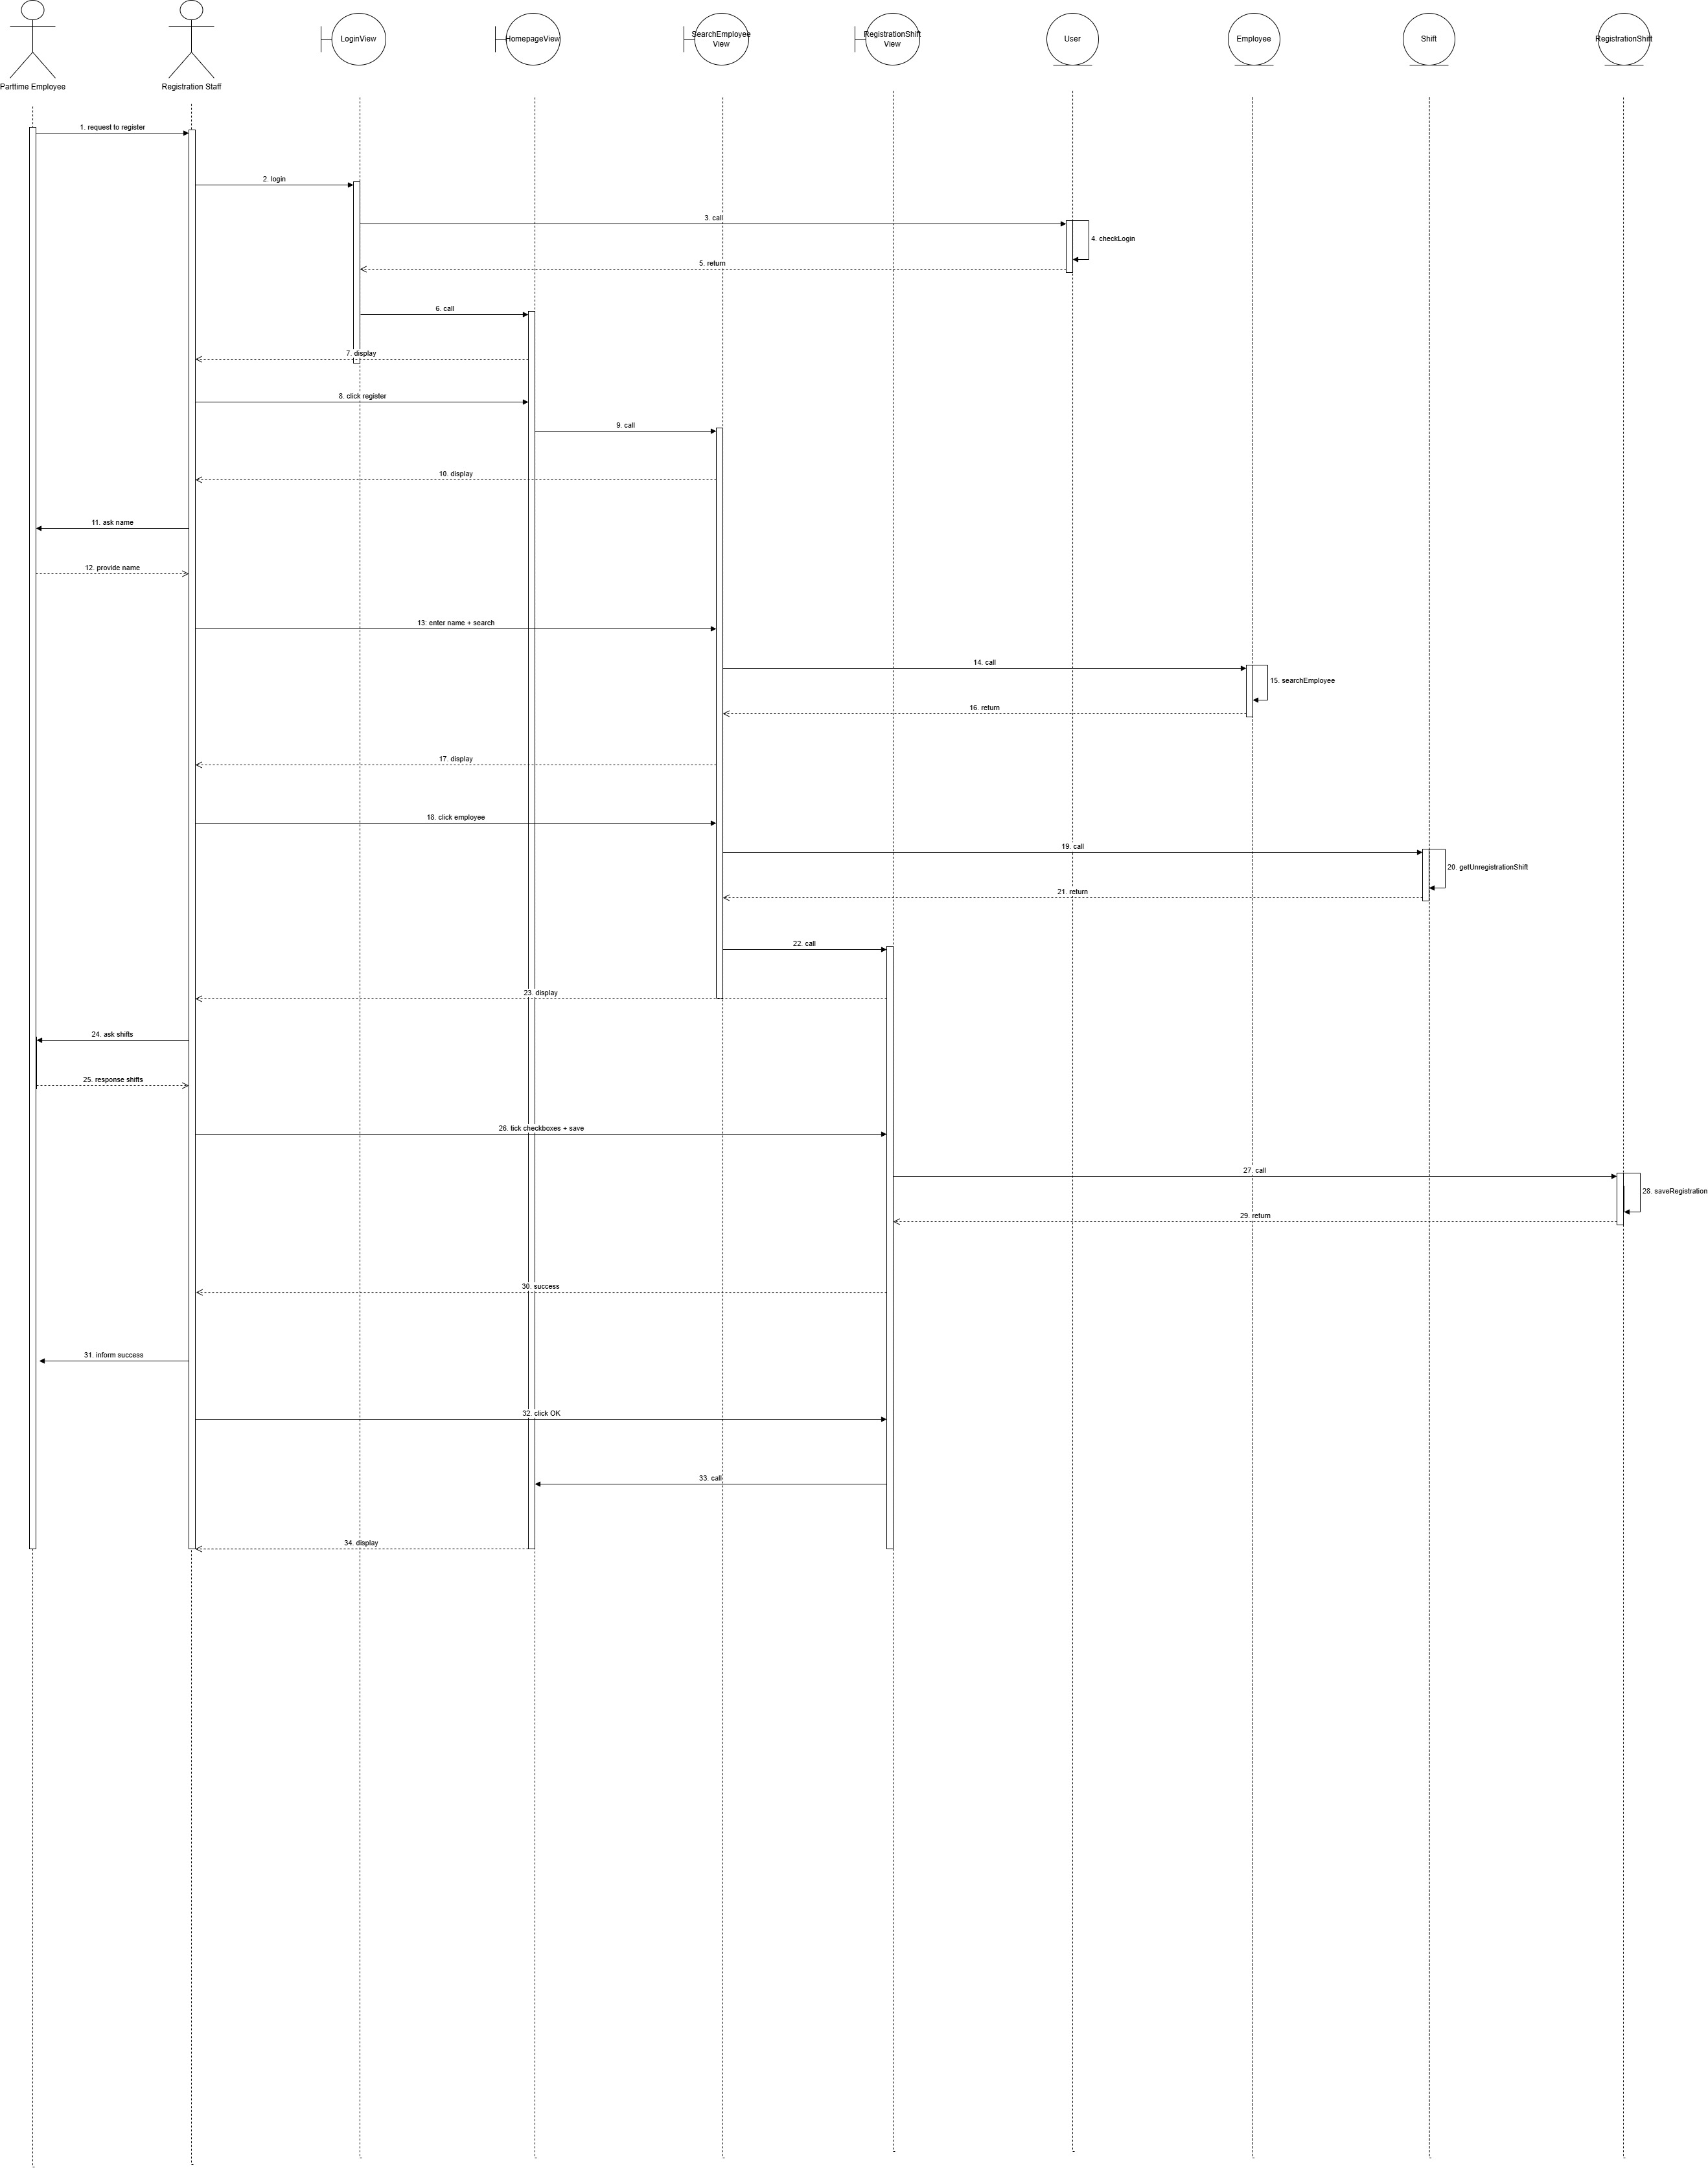
\includegraphics[width=1.0\textwidth]{assets/diagrams/Sequence Diagram.jpg}
    \caption{Sequence Diagram for the Standard Scenario of the Register Next Week Module}
    % \label{fig:sequence_diagram}
\end{figure}
